\section{Experiments}\label{sec:experiments}

\subsection{Data, predictors, and families}\label{sec:data}
We use the ProteinGym v1.3 clinical substitution benchmark~\cite{notin2023proteingym}: \nVariants{} ClinVar missense variants in \nProteins{} human proteins, \fracPath{} pathogenic, with a median of \medVar{} labeled variants per protein (maximum \maxVar{}). We take ProteinGym's precomputed zero-shot scores for five unsupervised predictors: ESM-1b (protein language model), EVE and GEMME (alignment-based), TranceptEVE (hybrid), and PoET (retrieval-augmented language model). We orient every score so that higher means more pathogenic, using ProteinGym's directionality settings; our per-protein mean AUCs agree with ProteinGym's published values (\pubAucRange{}) to three decimals. Supervised clinical predictors in the same files are excluded because they are trained on ClinVar.

Families are MMseqs2~\cite{steinegger2017mmseqs2} clusters of wild-type sequences at 30\% identity and 80\% bidirectional coverage: \nFam{} families, of which \nFamSingleton{} are single proteins (largest: \maxFamSize{} proteins) and \nFamGeTen{} have at least ten variants. As sensitivity checks we use 50\% identity (\nFamFifty{} families) and single-linkage components of significant homology ($E\le10^{-3}$, identity $\ge30\%$, both sequences covered $\ge50\%$; \nFamHC{} families), which merges homologs that share a domain. Family descriptors are computed without labels: maximum identity to any training protein over significant MMseqs2 hits, $\log N_{\mathrm{eff}}$ and $N_{\mathrm{eff}}$ per position from ProteinGym's alignment weights, cosine distance of mean-pooled ESM2-35M~\cite{lin2023evolutionary} embeddings to the nearest training protein, $\log$ length, $\log$ number of scored variants, and, for one ablation, summaries of the predictor's scores. A family is an \emph{orphan} if no member has a significant hit at $\ge30\%$ identity outside the family (\nFamOrphan{} families).

\subsection{Protocol}\label{sec:protocol}
Each of ten seeds splits families into 40\% training, 30\% calibration and 30\% test (\nTrainFam{}, \nCalFam{} and \nTestFam{} families). \textbf{S1} draws all three uniformly at random. \textbf{S2} keeps the S1 training families and samples test families without replacement with probability proportional to $\exp(-\beta z)$, where $z$ is the standardized mean of maximum identity to training and $\log N_{\mathrm{eff}}$, so that test families are poorly supported and calibration families well supported; $\beta\in\{0.5,1,2\}$ ($\beta=0$ is S1). At $\beta=1$, mean maximum identity to training is \sTwoTestMaxId{} for test and \sTwoCalMaxId{} for calibration families, and mean $\log N_{\mathrm{eff}}$ is \sTwoTestNeff{} against \sTwoCalNeff{}. \textbf{S3} draws test families only from orphan families, a natural shift with no explicit model (mean maximum identity \sThreeTestMaxId{} against \sThreeCalMaxId{}). \textbf{S4} holds out regions of protein space: $k$-means groups families into 20 regions by the leading principal components of their mean ESM2 embeddings, each seed takes whole regions in random order as test families (splitting the last one at random to reach the test size), and training and calibration families come from the remaining families. Unlike S2, this shift is defined in embedding space rather than by the scalar descriptors that $\hat w$ uses; held-out families are farther from training in embedding distance (\sFourTestEmb{} against \sFourCalEmb{}) and have deeper alignments (mean $\log N_{\mathrm{eff}}$ \sFourTestNeff{} against \sFourCalNeff{}).

The base model, fitted on training families only, is a logistic regression on the raw score (clipped to the training 0.1\% and 99.9\% quantiles) and the score standardized within its protein over the protein's scored variants (label-free, but it assumes the protein's variant panel is available; a deployment-realistic run without it, and without the variant-count descriptor, is in Section~\ref{sec:results}); its test AUC is \baseAucRange{} across predictors. Baselines are variant-level split conformal (B1) and its class-conditional version (B2); family-level HCP pooling and Dunn et al.'s single and repeated subsampling (B3)~\cite{lee2026hierarchical,dunn2023distribution}; group-weighted conformal (B4)~\cite{bhattacharyya2024group} with nine bins (maximum identity zero, low or high, crossed with $\log N_{\mathrm{eff}}$ terciles) and target proportions from the test families; and support-only and random abstention at ProtCOVER's abstention rate (B5). Every method has marginal and class-conditional versions. ProtCOVER uses \nCalConfFam{} of the calibration families in the quantile and the rest to fit $\hat w$. The gate's kernel scale is chosen by inner risk-coverage AUC and $(m,\pi_{\max})$ as the least-abstaining setting within 0.005 of the best retained coverage under a pre-declared 10\% abstention budget, all on a shifted ($\beta=1$) inner split of the training families. Test families are used only for final evaluation, and only their label-free descriptors enter $\hat w$. Appendix~\ref{app:protocol} lists all remaining settings.

We report family-weighted coverage $\Cov$, class-conditional $\Cov_1$ (pathogenic) and $\Cov_0$ (benign), variant-weighted coverage, mean set size, singleton rate, the fraction of families with at least ten variants whose coverage is below $1-\alpha-0.05$ (with its expectation under pure binomial noise), abstention rates, and risk-coverage curves (error of retained singleton sets against the retained fraction, abstaining whole families) with their area (AURC). Intervals are 95\% bootstrap intervals that resample test families within each seed and average over seeds; differences between methods use the same resamples (paired). Unless stated otherwise $\alpha=0.1$; results at $\alpha\in\{0.05,0.2\}$ are in Appendix~\ref{app:tables}.

\subsection{Results}\label{sec:results}

\begin{figure}[t]
\centering
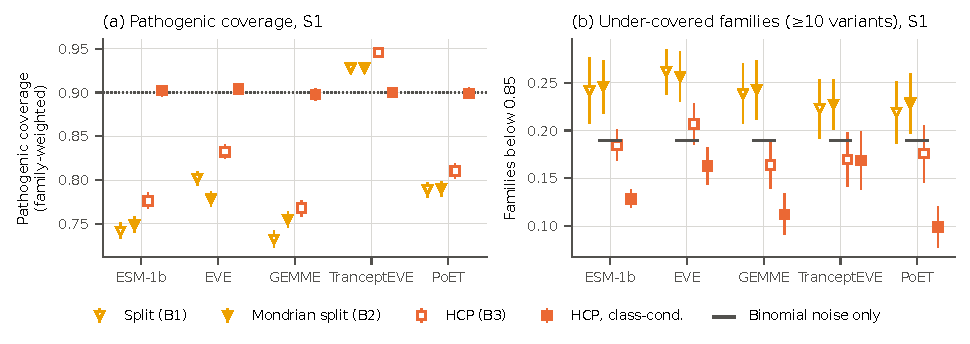
\includegraphics[width=\textwidth]{../figures/fig1_s1_family_coverage.pdf}
\caption{Exchangeable families (S1, $\alpha=0.1$). (a) Family-weighted pathogenic coverage $\Cov_1$ with 95\% family-bootstrap intervals; the dotted line is the target. (b) Fraction of families with at least ten variants whose overall coverage (both classes, for every method) is below 0.85 (mean and s.d. over seeds); the gray dash is the expected fraction if every family had coverage exactly 0.90.}
\label{fig:s1}
\end{figure}

\paragraph{Variant-level calibration misses pathogenic variants per family.}
In S1 (Fig.~\ref{fig:s1}), variant-level split conformal has variant-weighted coverage \sOneBoneCovVar{}, close to its target, but family-weighted coverage \sOneBoneCovFam{}; family-level HCP restores \sOneHcpCovFam{}. The gap is concentrated in the pathogenic class: B2, calibrated class by class over variants, attains variant-weighted pathogenic coverage \sOneBtwoPathVar{} for four predictors yet covers only \sOneBtwoPath{} of pathogenic variants per family. The 5\% of test families with the most pathogenic variants hold \sizeTopShare{} of them, and their pathogenic variants are easier: under B2, families with fewer than five pathogenic variants have pathogenic coverage \sizeCovFew{} against \sizeCovMany{} for families with at least twenty. TranceptEVE is the exception (\sOneBtwoPathTrancept{}), with the error moved to the benign class. Family-level class-conditional calibration attains \sOneHcpccPath{} (pathogenic) and \sOneHcpccBenign{} (benign), as Propositions~\ref{prop:hcp} and~\ref{prop:mondrian} guarantee, and lowers the fraction of under-covered families below the binomial-noise level (Fig.~\ref{fig:s1}b), at the cost of larger sets.

\begin{figure}[t]
\centering
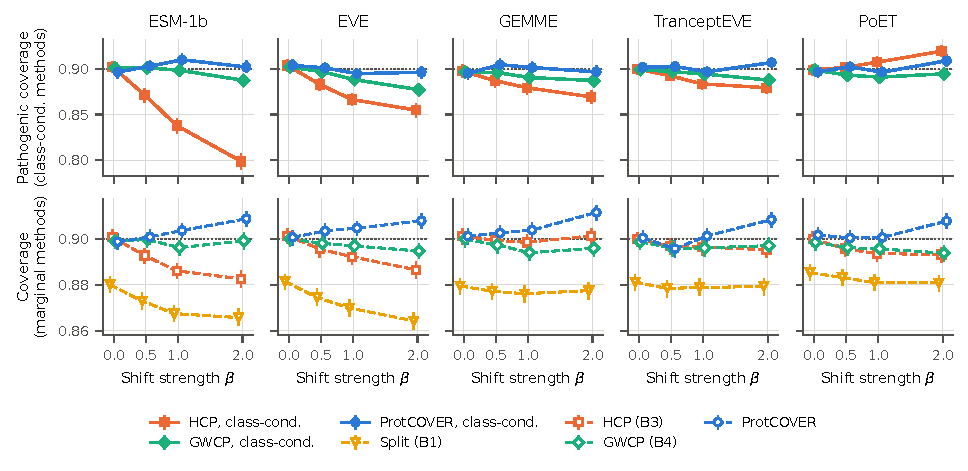
\includegraphics[width=\textwidth]{../figures/fig2_shift_sweep.pdf}
\caption{Coverage under increasing descriptor shift (S2; $\beta=0$ is S1), $\alpha=0.1$, with 95\% family-bootstrap intervals; methods are offset slightly in $\beta$. Top: pathogenic coverage $\Cov_1$ of class-conditional family-level methods (Mondrian split, far below the target for four predictors, is in Table~\ref{tab:main}). Bottom: family-weighted coverage $\Cov$ of marginal methods.}
\label{fig:shift}
\end{figure}

\begin{table}[t]
\caption{Family-weighted pathogenic / benign coverage ($\Cov_1$ / $\Cov_0$) of class-conditional methods at $\alpha=0.1$ (target 0.90), mean over ten seeds. The ProtCOVER row omits the gate, which can only raise coverage (Lemma~\ref{lem:enlarge}); the full method is in Table~\ref{tab:ablation}. Paired differences with intervals are in Table~\ref{tab:paired}.}
\label{tab:main}
\centering\scriptsize\setlength{\tabcolsep}{3pt}
\begin{tabular}{llccccc}
\toprule
Setting & Method & ESM-1b & EVE & GEMME & TranceptEVE & PoET \\
\midrule
S1 (exchangeable) & Mondrian split (B2) & 0.749 / 0.899 & 0.778 / 0.898 & 0.755 / 0.895 & 0.928 / 0.837 & 0.790 / 0.877 \\
 & HCP (B3) & 0.903 / 0.903 & 0.904 / 0.901 & 0.898 / 0.898 & 0.900 / 0.901 & 0.899 / 0.903 \\
 & GWCP (B4) & 0.902 / 0.901 & 0.902 / 0.899 & 0.897 / 0.897 & 0.900 / 0.900 & 0.899 / 0.901 \\
 & ProtCOVER & \textbf{0.897 / 0.904} & \textbf{0.904 / 0.902} & \textbf{0.895 / 0.899} & \textbf{0.902 / 0.902} & \textbf{0.897 / 0.906} \\
\midrule
S2, $\beta=1$ & Mondrian split (B2) & 0.655 / 0.929 & 0.709 / 0.915 & 0.712 / 0.906 & 0.920 / 0.839 & 0.795 / 0.856 \\
 & HCP (B3) & 0.838 / 0.927 & 0.867 / 0.916 & 0.879 / 0.909 & 0.884 / 0.894 & 0.908 / 0.875 \\
 & GWCP (B4) & 0.899 / 0.904 & 0.888 / 0.909 & 0.891 / 0.904 & 0.895 / 0.894 & 0.891 / 0.897 \\
 & ProtCOVER & \textbf{0.910 / 0.905} & \textbf{0.895 / 0.909} & \textbf{0.902 / 0.908} & \textbf{0.897 / 0.898} & \textbf{0.897 / 0.905} \\
\midrule
S2, $\beta=2$ & Mondrian split (B2) & 0.619 / 0.941 & 0.686 / 0.917 & 0.700 / 0.910 & 0.921 / 0.839 & 0.806 / 0.840 \\
 & HCP (B3) & 0.798 / 0.939 & 0.855 / 0.917 & 0.869 / 0.914 & 0.880 / 0.891 & 0.920 / 0.853 \\
 & GWCP (B4) & 0.888 / 0.905 & 0.877 / 0.906 & 0.887 / 0.897 & 0.888 / 0.889 & 0.895 / 0.873 \\
 & ProtCOVER & \textbf{0.902 / 0.915} & \textbf{0.896 / 0.916} & \textbf{0.898 / 0.915} & \textbf{0.908 / 0.900} & \textbf{0.910 / 0.892} \\
\midrule
S3 (orphan families) & Mondrian split (B2) & 0.678 / 0.915 & 0.772 / 0.895 & 0.724 / 0.903 & 0.943 / 0.823 & 0.817 / 0.854 \\
 & HCP (B3) & 0.876 / 0.908 & 0.909 / 0.899 & 0.890 / 0.905 & 0.914 / 0.892 & 0.931 / 0.879 \\
 & GWCP (B4) & 0.889 / 0.905 & 0.903 / 0.898 & 0.895 / 0.900 & 0.903 / 0.913 & 0.901 / 0.900 \\
 & ProtCOVER & \textbf{0.894 / 0.908} & \textbf{0.907 / 0.901} & \textbf{0.900 / 0.908} & \textbf{0.900 / 0.921} & \textbf{0.901 / 0.910} \\
\bottomrule
\end{tabular}

\end{table}

\paragraph{Weighting restores coverage under family-level shift.}
Under S2 (Fig.~\ref{fig:shift}, Table~\ref{tab:main}), family-level calibration alone degrades as $\beta$ grows: at $\beta=1$ its pathogenic coverage spans \sTwoBoneHcpPath{} across predictors, and for ESM-1b it falls to \sTwoBtwoHcpPathEsm{} at $\beta=2$. Its error is not one-sided: for PoET, and for TranceptEVE in S3, it over-covers pathogenic variants while under-covering benign ones. We therefore score each method by the shortfall of its worse class below the target. Over the \nShiftCells{} shifted predictor-setting cells (S2 with $\beta>0$, S3, and S4), this shortfall averages \shortHcpMean{} for HCP (maximum \shortHcpMax{}; worse class below 0.89 in \shortHcpN{} cells), \shortGwcpMean{} for GWCP (\shortGwcpMax{}; \shortGwcpN{} cells), and \shortPwMean{} for ProtCOVER (\shortPwMax{}; \shortPwN{} cells). Both components matter: the same weights applied to variant-level calibration leave a mean shortfall of \shortVarWMean{} (Table~\ref{tab:ablation}). GWCP, whose bins use the two descriptors that define the S2 shift, is the strongest baseline; at $\beta=2$ ProtCOVER's pathogenic coverage exceeds it by \sTwoBtwoDiffGwcp{} with paired intervals above zero for \sTwoBtwoDiffGwcpNpos{} of 5 predictors (Appendix Table~\ref{tab:paired}). S2 favors weighting by construction, since it shifts the very descriptors that $\hat w$ models. On the natural shift of S3, ProtCOVER only matches GWCP (differences \sThreeDiffGwcp{}), while still correcting HCP's errors in both directions. On held-out regions of embedding space (S4), variant-level Mondrian calibration again covers only \sFourBtwoPathNT{} of pathogenic variants per family for four predictors, but family-level calibration alone is already close to the target (worse-class shortfall \shortHcpFourMean{}, maximum \shortHcpFourMax{}), and weighting brings no gain: ProtCOVER's shortfall is \shortPwFourMean{} (maximum \shortPwFourMax{}) against \shortGwcpFourMean{} for GWCP. With little bias left to correct, the estimated weights mainly add variance; in S4, looser clipping lowers coverage (Table~\ref{tab:ablation}). The fraction of under-covered families is similar for the three family-level methods under shift (ProtCOVER \underPwShift{}, GWCP \underGwcpShift{}, HCP \underHcpShift{}; binomial-noise reference \underNullShift{}). Our bootstrap intervals are conditional on the splits; across seeds, ProtCOVER's pathogenic coverage in a cell has standard deviation \seedSdPwPath{}, so differences of about 0.01 between methods should be read with care. The price is larger sets (Fig.~\ref{fig:tradeoff}): averaged over the shifted cells, mean set size is \sizePwShift{} for ProtCOVER, \sizeGwcpShift{} for GWCP and \sizeHcpShift{} for HCP, and ProtCOVER returns both labels for \fullPwRange{} of variants, depending on predictor and setting. At matched pathogenic coverage of 0.90, interpolated along the $\alpha$ curves, the three methods need the same mean set size (\sizeMatchedPw{}, \sizeMatchedGwcp{} and \sizeMatchedHcp{} over the \nMatched{} cells where all three reach 0.90), and paired differences in singleton error at $\alpha=0.1$ are small and of both signs (\diffSingErrGwcp{} against GWCP; Appendix Table~\ref{tab:efficiency}). The extra size thus buys coverage along a shared coverage-size trade-off; it neither costs nor gains efficiency.

\begin{figure}[t]
\centering
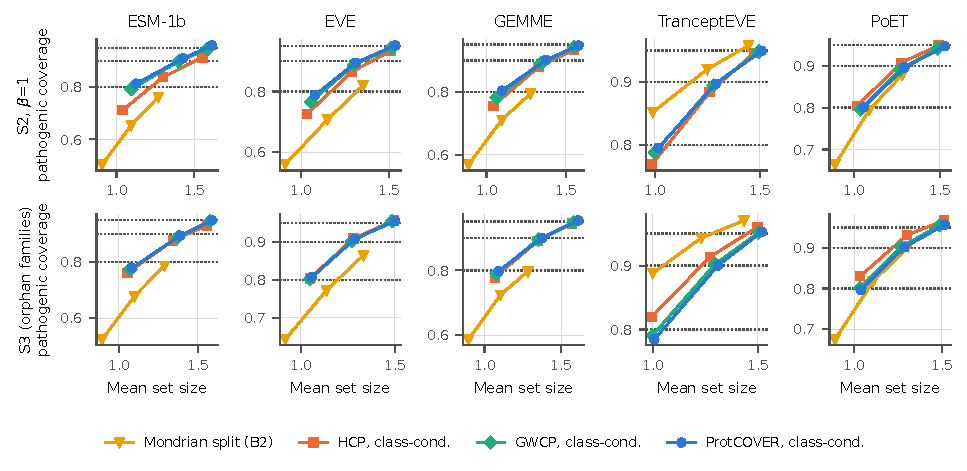
\includegraphics[width=\textwidth]{../figures/fig3_coverage_size.pdf}
\caption{Pathogenic coverage against mean set size for $\alpha\in\{0.2,0.1,0.05\}$ (left to right along each curve), class-conditional methods. Dotted lines mark the three targets.}
\label{fig:tradeoff}
\end{figure}

\paragraph{Summary across shifts.}
Under the natural shifts, family-level calibration does most of the work and weighting is neutral: ProtCOVER minus GWCP in pathogenic coverage spans \sThreeDiffGwcp{} in S3 and \sFourDiffGwcp{} in S4. Under descriptor shift (S2), weighting adds a clear gain with paired intervals above zero. Differences below about 0.01 are within seed-to-seed variation, and since all seeds resplit one pool of families, these conclusions are limited to this benchmark.

\paragraph{The support gate preserves coverage but does not improve selective risk.}
With $(m,\pi_{\max})$ and the kernel scale tuned on training families under a 10\% budget, the gate abstained on at most \gateAbsMaxNoBtwo{} of test families except at $\beta=2$ (\gateAbsBtwo{}), so the full method matches (i)+(ii) (Table~\ref{tab:ablation}). The 10\% budget is a cap: tuning chose so little abstention because abstaining more did not raise retained coverage on the inner split. Risk-coverage curves (Appendix Fig.~\ref{fig:risk}) evaluate the ranking itself at every abstention level, against random abstention averaged over 100 random family orders. Abstaining first on the families with the lowest ESS gave a lower AURC than random abstention in the majority of seeds in \riskEssNBetter{} of \riskNCells{} predictor-setting cells and a higher one in \riskEssNWorse{} (the rest tied); ranking by maximum identity (\riskSupportNBetter{} lower, \riskSupportNWorse{} higher) or by test-point mass (\riskMassNBetter{} lower, \riskMassNWorse{} higher) did no better. On this benchmark, how well a family is supported by calibration data does not predict how often the predictor errs on it once coverage is controlled. The gate therefore adds nothing measurable here; Lemma~\ref{lem:enlarge} guarantees only that it costs no coverage.


\begin{table}[t]
\caption{Ablations: pathogenic coverage $\Cov_1$ at $\alpha=0.1$, mean (minimum) over the five predictors. For family definitions, HCP / ProtCOVER.}
\label{tab:ablation}
\centering\scriptsize\setlength{\tabcolsep}{3pt}
\begin{tabular}{lcccc}
\toprule
Configuration & S2, $\beta=1$ & S2, $\beta=2$ & S3 & S4 \\
\midrule
\multicolumn{5}{l}{\emph{Components}} \\
(i) family-level calibration (HCP) & 0.875 (0.838) & 0.864 (0.798) & 0.904 (0.876) & 0.904 (0.891) \\
(i)+(ii), conditional on $\hat w$ (ProtCOVER) & 0.901 (0.897) & 0.925 (0.920) & 0.902 (0.890) & 0.914 (0.912) \\
(i)+(ii), conditional on descriptors (ProtCOVER-D) & 0.901 (0.898) & 0.902 (0.890) & 0.905 (0.894) & 0.902 (0.885) \\
(i)+(ii), reweighting by $\hat w$ (ProtCOVER-W) & 0.900 (0.895) & 0.902 (0.896) & 0.900 (0.894) & 0.895 (0.886) \\
(i)+(iii) gate & 0.875 (0.838) & 0.864 (0.798) & 0.904 (0.876) & 0.904 (0.891) \\
ProtCOVER-W + (iii) gate & 0.900 (0.895) & 0.904 (0.898) & 0.901 (0.894) & 0.895 (0.886) \\
(ii) without (i): variant-level weighting & 0.789 (0.740) & 0.787 (0.723) & 0.807 (0.740) & 0.798 (0.737) \\
\multicolumn{5}{l}{\emph{Descriptors for $\hat w$ (ProtCOVER-W)}} \\
sequence similarity only & 0.871 (0.850) & 0.853 (0.799) & 0.899 (0.892) & 0.906 (0.903) \\
alignment depth only & 0.899 (0.892) & 0.901 (0.872) & 0.899 (0.878) & 0.903 (0.893) \\
embedding distance only & 0.879 (0.845) & 0.866 (0.806) & 0.904 (0.872) & 0.895 (0.882) \\
the three support groups & 0.900 (0.894) & 0.904 (0.898) & 0.900 (0.894) & 0.896 (0.887) \\
main set + predictor score summaries & 0.903 (0.894) & 0.898 (0.889) & 0.902 (0.895) & 0.894 (0.887) \\
\multicolumn{5}{l}{\emph{Weight clipping $c$ (default 20; ProtCOVER-W)}} \\
$c=5$ & 0.899 (0.894) & 0.889 (0.870) & 0.900 (0.892) & 0.904 (0.897) \\
$c=100$ & 0.900 (0.895) & 0.908 (0.904) & 0.901 (0.894) & 0.883 (0.874) \\
no clipping & 0.900 (0.895) & 0.908 (0.904) & 0.901 (0.894) & 0.837 (0.779) \\
\bottomrule
\end{tabular}

\end{table}

\paragraph{Ablations.}
Table~\ref{tab:ablation} shows that sequence similarity or embedding distance alone does not correct the S2 shift, alignment depth alone helps on average but not for every predictor, and the support descriptors together match the full set; adding the predictor's score summaries does not help and lowers the worst predictor's coverage at $\beta=2$. Embedding distance contributes little here because it barely differs between calibration and test families (mean \sTwoCalEmb{} against \sTwoTestEmb{} at $\beta=1$). Tight clipping ($c=5$) under-corrects at $\beta=2$, while loose or no clipping hurts in S4, so the clipping level trades bias correction against variance. Under the alternative family definitions, ProtCOVER's mean pathogenic coverage over predictors stays at \sensPwMeanRange{} across the shifted settings; its worst predictor-setting cell is \sensFiftyPwMin{} with 50\% clustering and \sensHcPwMin{} with homology components, against \sensFiftyHcpMin{} and \sensHcHcpMin{} for HCP.

\paragraph{Deployment-realistic features.}
The base model's within-protein standardization and the variant-count descriptor both need the query protein's whole variant panel. Without them (raw score only, no variant count; Table~\ref{tab:ablation}), Mondrian split still covers only \realBtwoPath{} of pathogenic variants per family in S1, below the target for \realBtwoNBelow{} of 5 predictors, and the ranking under shift is unchanged: mean worse-class shortfall \realShortPwMean{} for ProtCOVER, \realShortGwcpMean{} for GWCP and \realShortHcpMean{} for HCP (worst coverage \realWorstPw{}, \realWorstGwcp{} and \realWorstHcp{}). Sets are smaller for every method, for example \realSizePw{} for ProtCOVER against \sizePwShift{} with the full features.

\subsection{Synthetic validation}\label{sec:synthetic}
On simulated families where A1 or A2 hold exactly (Appendix~\ref{app:synthetic}), family-weighted coverage at a 0.90 target is \synHcpEasy{} for family-level and \synBoneEasy{} for variant-level calibration, and under a strong family-level shift ($\beta=2$) weighting with cross-fitted estimated ratios attains \synShiftTwoEst{} where family-level calibration alone falls to \synShiftTwoHcp{}.
